%% LyX 2.1.4 created this file.  For more info, see http://www.lyx.org/.
%% Do not edit unless you really know what you are doing.
\documentclass[oneside,english]{amsart}
\usepackage[T1]{fontenc}
\usepackage[latin9]{inputenc}
\usepackage{geometry}
\geometry{verbose,tmargin=1cm,bmargin=1cm,lmargin=1cm,rmargin=1cm,headheight=1cm,headsep=1cm,footskip=1cm}
\usepackage{float}
\usepackage{amstext}
\usepackage{amsthm}
\usepackage{amssymb}
\usepackage{graphicx}
\usepackage{esint}

\makeatletter

%%%%%%%%%%%%%%%%%%%%%%%%%%%%%% LyX specific LaTeX commands.
\floatstyle{ruled}
\newfloat{algorithm}{tbp}{loa}
\providecommand{\algorithmname}{Algorithm}
\floatname{algorithm}{\protect\algorithmname}

%%%%%%%%%%%%%%%%%%%%%%%%%%%%%% Textclass specific LaTeX commands.
\numberwithin{equation}{section}
\numberwithin{figure}{section}

\makeatother

\usepackage{babel}
\usepackage{listings}
\renewcommand{\lstlistingname}{Listing}

\begin{document}

\title{MAD6406 Homework Fall 2015}


\author{Maksim Levental}
\maketitle
\begin{enumerate}
\item [1.3] Claim: $R$ upper triangular and nonsingular iff $R^{-1}$
upper triangular.

\begin{proof}
$R$ nonsingular implies all diagonal entries of $R$ are non-zero.
Therefore for $n<m$ the span of $\left\{ r_{1},\dots,r_{n}\right\} $,
where $r_{i}$ are the columns of $R$, is $\mathbb{R}^{n}$. Therefore
there exist $\rho_{jn}$ for $j=1,\dots,n$ such that 
\[
r_{1}\rho_{1n}+r_{2}\rho_{2n}+\cdots+r_{n}\rho_{nn}=e_{n}
\]
Let $\rho_{jn}=0$ for $n<j<\leq m$ and hence 
\[
r_{1}\rho_{1n}+r_{2}\rho_{2n}+\cdots+r_{m}\rho_{mn}=e_{n}
\]
Then let 
\[
\rho_{i}=\begin{bmatrix}\rho_{1i}\\
\vdots\\
\rho_{ii}\\
\vdots\\
\rho_{mi}
\end{bmatrix}=\begin{bmatrix}\rho_{1i}\\
\vdots\\
\rho_{ii}\\
0\\
\vdots\\
0
\end{bmatrix}
\]
and $P=\begin{bmatrix}\rho_{1} & \cdots & \rho_{m}\end{bmatrix}$.
Note that $P$ is upper-triangular since for all $i$ it's the case
that $\rho_{jn}=0$ for $j=n+1,\cdots,m$. Furthermore by \ref{eq:uppertriang}
we have that $R\cdot P=I$ and by uniqueness of inverses $P=R^{-1}$. 
\end{proof}
\item [2.3] Claim: for self-adjoint $A\in\mathbb{C}^{m\times m}$

\begin{enumerate}
\item All eigenvalues of $A$ are real.
\item Eigenvectors corresponding to distinct eigenvalues are orthogonal.\end{enumerate}
\begin{proof}

\begin{enumerate}
\item Let $x\neq0$ and $\lambda$ such that $Ax=\lambda x$. Then by self-adjointness
\[
\left(x^{\dagger}Ax\right)^{\dagger}=\left(\left(Ax\right)^{\dagger}\left(x^{\dagger}\right)^{\dagger}\right)=\left(x^{\dagger}A^{\dagger}x\right)=\left(x^{\dagger}Ax\right)
\]
but
\[
x^{\dagger}Ax=x^{\dagger}\lambda x=\lambda\left\Vert x\right\Vert ^{2}
\]
and $\lambda\left\Vert x\right\Vert ^{2}=\left(\lambda\left\Vert x\right\Vert ^{2}\right)^{\dagger}=\lambda^{*}\left\Vert x\right\Vert ^{2}$.
Therefore $\lambda=\lambda^{*}$ hence $\lambda\in\mathbb{R}$.
\item Let $x\neq y\neq0$ and $\lambda,\lambda^{'}$ such that$Ax=\lambda x$
and $Ay=\lambda^{'}y$. Then by self-adjointness
\[
x^{\dagger}Ay=\left(Ax\right)^{\dagger}y
\]
and so since $\lambda,\lambda^{'}\in\mathbb{R}$ 
\[
0=x^{\dagger}Ay-\left(Ax\right)^{\dagger}y=\lambda^{'}x^{\dagger}y-\lambda x^{\dagger}y=\left(\lambda^{'}-\lambda\right)x^{\dagger}y
\]
Therefore since $\lambda\neq\lambda^{'}$ it's the case that $\lambda^{'}-\lambda\neq0$
and hence $x^{\dagger}y=0$.
\end{enumerate}
\end{proof}
\item [3.5]Claim: $\left\Vert A\right\Vert _{F}=\left\Vert uv^{*}\right\Vert _{F}=\left\Vert u\right\Vert _{F}\left\Vert v\right\Vert _{F}$.

\begin{proof}
Since the Frobenius norm of a vector is just the 2-norm so it distributes
over the product. To wit if $A=uv^{*}$ 
\[
\left\Vert A\right\Vert _{F}=\left\Vert uv^{*}\right\Vert _{F}=\sqrt{\sum_{i,j}\left|u_{j}v_{i}^{*}\right|^{2}}=\sqrt{\sum_{j}\left|u_{j}\right|^{2}\sum_{i}\left|v_{i}^{*}\right|^{2}}=\sqrt{\sum_{j}\left|u_{j}\right|^{2}}\sqrt{\sum_{i}\left|v_{i}^{*}\right|^{2}}
\]
Now since $\left|x^{*}\right|=\left|x\right|$
\[
\sqrt{\sum_{j}\left|u_{j}\right|^{2}}\sqrt{\sum_{i}\left|v_{i}^{*}\right|^{2}}=\sqrt{\sum_{j}\left|u_{j}\right|^{2}}\sqrt{\sum_{i}\left|v_{i}\right|^{2}}=\left\Vert u\right\Vert _{F}\left\Vert v\right\Vert _{F}
\]

\end{proof}
\item [4.4]Claim: it is \textbf{false }that $A,B\in\mathbb{C}^{m}$ are
unitary equivalent iff they have the same singular values.

\begin{proof}
$A$ and $-A$ have the same singular values: let $A=U\Sigma V^{-1}$,
then 
\[
-A=U\Sigma\left(-V^{-1}\right)
\]
But $A$ and $-A$ cannot be unitarily equivalent since then 
\begin{eqnarray*}
\det\left(A\right) & = & \det\left(Q\left(-A\right)Q^{-1}\right)\\
 & = & \det\left(Q\right)\det\left(-A\right)\det\left(Q^{-1}\right)\\
 & = & \det\left(Q\right)\det\left(Q^{-1}\right)\det\left(-A\right)\\
 & = & \left(-1\right)^{m}\det\left(A\right)
\end{eqnarray*}
which is only true if $m$ is even or $\det\left(A\right)=0$. Alternatively
\begin{eqnarray*}
\text{tr}\left(A\right) & = & \text{tr}\left(Q\left(-A\right)Q^{-1}\right)\\
 & = & \text{tr}\left(Q^{-1}Q\left(-A\right)\right)\\
 & = & -\text{tr}\left(A\right)
\end{eqnarray*}
which is only true if $\left(A\right)_{ii}=0$ for all $i$.
\end{proof}
\item [5.4]Claim: if $A\in\mathbb{C}^{m\times m}$, with $A=U\Sigma V^{-1}=U\Sigma V^{\dagger}$,
and 
\[
B=\begin{pmatrix}0 & A^{\dagger}\\
A & 0
\end{pmatrix}
\]
then there exists $X,\Lambda$ such that $B=X\Lambda X^{-1}$ is an
eigenvalue decomposition.

\begin{proof}
First note that $A^{\dagger}=\left(U\Sigma V^{\dagger}\right)^{\dagger}=V\Sigma^{\dagger}U^{\dagger}=V\Sigma U^{\dagger}$
since singular values are always real\footnote{Thm. 4.1 in Trefethen: $\sigma_{1}=\left\Vert A\right\Vert $}.
Since $A$ is square 
\begin{eqnarray*}
A^{\dagger}u_{j} & = & \sigma_{j}v_{j}\\
Av_{j} & = & \sigma_{j}u_{j}
\end{eqnarray*}
Hence 
\[
B\begin{pmatrix}u_{j}\\
v_{j}
\end{pmatrix}=\begin{pmatrix}0 & A^{\dagger}\\
A & 0
\end{pmatrix}\begin{pmatrix}v_{j}\\
u_{j}
\end{pmatrix}=\begin{pmatrix}A^{\dagger}u_{j}\\
Av_{j}
\end{pmatrix}=\begin{pmatrix}\sigma_{j}v_{j}\\
\sigma_{j}u_{j}
\end{pmatrix}=\sigma_{j}\begin{pmatrix}v_{j}\\
u_{j}
\end{pmatrix}
\]
and 
\[
B\begin{pmatrix}v_{j}\\
-u_{j}
\end{pmatrix}=\begin{pmatrix}0 & A^{\dagger}\\
A & 0
\end{pmatrix}\begin{pmatrix}v_{j}\\
-u_{j}
\end{pmatrix}=\begin{pmatrix}-A^{\dagger}u_{j}\\
Av_{j}
\end{pmatrix}=\begin{pmatrix}-\sigma_{j}v_{j}\\
\sigma_{j}u_{j}
\end{pmatrix}=-\sigma_{j}\begin{pmatrix}v_{j}\\
-u_{j}
\end{pmatrix}
\]
Therefore the eigenvectors of $B$ are $\left\{ \begin{pmatrix}v_{1}\\
u_{1}
\end{pmatrix},\dots,\begin{pmatrix}v_{m}\\
u_{m}
\end{pmatrix},\begin{pmatrix}v_{1}\\
-u_{1}
\end{pmatrix},\dots,\begin{pmatrix}v_{m}\\
-u_{m}
\end{pmatrix}\right\} $ with eigenvalues $\left\{ \sigma_{1},\dots,\sigma_{m},-\sigma_{1},\dots,-\sigma_{m}\right\} $
and hence 
\[
B=\begin{pmatrix}V & V\\
U & -U
\end{pmatrix}\begin{pmatrix}\Sigma & 0\\
0 & -\Sigma
\end{pmatrix}\begin{pmatrix}V & V\\
U & -U
\end{pmatrix}^{-1}
\]

\end{proof}
\item [6.1]Claim: if $P$ is an orthogonal projector, the $I-2P$ is unitary.

\begin{proof}
Since $P$ is an orthogonal projector $P=P^{\dagger}$ and hence 
\begin{eqnarray*}
\left(I-2P\right)^{\dagger}\left(I-2P\right) & = & \left(I^{\dagger}-2P^{\dagger}\right)\left(I-2P\right)\\
 & = & \left(I-2P\right)\left(I-2P\right)\\
 & = & I-4P-4P^{2}\\
 & = & I-4P-4P\\
 & = & I
\end{eqnarray*}
Hence $P$ is unitary. The geometric intuition is that since $I-2P=\left(I-P\right)-P$
it's the case that 
\begin{eqnarray*}
\left(I-2P\right)x & = & \left(I-P\right)x-Px
\end{eqnarray*}
Since in general $x=\left(I-P\right)x+Px$ it's obvious that $\left(I-P\right)x+\left(-Px\right)$
is the reflection of $x$ across $\text{range}\left(I-P\right)$,
which is what unitary transformations are (reflections and/or rotations).
\end{proof}
\item [7.4]Let $P_{1}=\left[x^{\left(1\right)},y^{\left(1\right)}\right]$
and $P_{2}=\left[x^{\left(2\right)},y^{\left(2\right)}\right]$ be
matrices. Then compute the full QR factorizations $P_{1}=Q_{1}R_{1}$
and $P_{2}=Q_{2}R_{2}$. The third columns $z^{\left(1\right)},z^{\left(2\right)}$of
$Q_{1},Q_{2}$ are orthogonal to $P^{\left(1\right)},P^{\left(2\right)}$
respectively. Then let matrix $P_{3}=\left[z^{\left(1\right)},z^{\left(2\right)}\right]$
and $P_{3}=Q_{3}R_{3}$. Then the third column $z^{\left(3\right)}$
of $Q_{3}$ is orthogonal to $\left\langle z^{\left(1\right)},z^{\left(2\right)}\right\rangle $,
i.e. in both $P^{\left(1\right)}$ and $P^{\left(2\right)}$.\\
\\
\\

\item [8.2]MATLAB QR factorization code appears in algorithm \ref{alg:Problem-8.2}.
\begin{algorithm}[h]
\noindent \centering{}
\begin{lstlisting}[language=Matlab,basicstyle={\footnotesize},showstringspaces=false,tabsize=2]
function [ Q,R ] = mgs( A )

n=size(A,2); 
V = A; 
R = zeros(n); 
Q = zeros(size(A));
for i=1:n
    R(i,i) = norm(V(:,i));
    Q(:,i) = V(:,i)/R(i,i);
    for j=i+1:n
        R(i,j) = dot(conj(Q(:,i)),V(:,j));
        V(:,j) = V(:,j) - R(i,j)*Q(:,i);
    end
end
\end{lstlisting}
\caption{Problem 8.2\label{alg:Problem-8.2}}
\end{algorithm}

\item [10.2]

\begin{enumerate}
\item MATLAB QR factorization by Householder orthogonal triangularization
code appears in algorithm \ref{alg:Problem-10.2(a)}. 
\begin{algorithm}[h]
\begin{lstlisting}[language=Matlab,basicstyle={\footnotesize},tabsize=2]
function [W,R] = house( A )
%HOUSE computes implicit representation of QR using householder
%orthogonal trianglurization
[m,n]=size(A);
W=zeros([m,n]);
R=A;
for k=1:n
    x = R(k:m,k);
    vk = sign(x(1))*norm(x)*vertcat(1,zeros(m-k,1)) + x;
    vk = vk/norm(vk);
    W(k:m,k) = vk;
    R(k:m,k:n) = R(k:m,k:n) - 2*vk*(vk'*R(k:m,k:n));
end
end
\end{lstlisting}


\caption{Problem 10.2(a)\label{alg:Problem-10.2(a)}}
\end{algorithm}

\item Reconstruction of Q from Householder decomposition code appears in
algorithm \ref{alg:Problem-10.2(b)}.
\begin{algorithm}[h]
\begin{lstlisting}[language=Matlab,basicstyle={\footnotesize},tabsize=2]
function Q=formQ(W)
%formQ reconstructs Q from W by computing Qe_i for i=1,..,m
[m,n]=size(W);
Q=eye(m);
for j=1:m
    for k=n:-1:1
        Q(k:m,j) = Q(k:m,j) - 2*W(k:m,k)*(W(k:m,k)'*Q(k:m,j));
    end
end
end
\end{lstlisting}


\caption{Problem 10.2(b)\label{alg:Problem-10.2(b)}}
\end{algorithm}

\end{enumerate}
\item [11.3] Experimentation MATLAB code appears in algorithm \ref{alg:Problem-11.3}.
\begin{algorithm}[h]
\begin{lstlisting}[language=Matlab,basicstyle={\footnotesize},showstringspaces=false,tabsize=2]
m=50;n=12;
t=linspace(0,1,m);
A=fliplr(vander(t));
A=A(:,1:n);
b=cos(4*t);
% (a)
xa = (A'*A)\(A'*b');
% (b)
[Q,R]=mgs(A);
xb = inv(R)*Q'*b';
% (c)
[Q,~,R]=house(A);
xc = inv(R(1:n,:))*Q(:,1:n)'*b';
% (d)
[Q,R]=qr(A,0); xd = inv(R)*Q'*b';
% (e) xe = A\b';
% (f)
[U,S,V] = svd(A,0); xf = V*inv(S)*U';
\end{lstlisting}


\caption{Problem 11.3\label{alg:Problem-11.3}}
\end{algorithm}
Results appear below. spurious digits are bolded (since I don't have
a color printer): {\scriptsize{}
\[
\begin{bmatrix}\left(a\right) & \left(b\right) & \left(c\right) & \left(d\right) & \left(e\right) & \left(f\right)\\
1.00000000\mathbf{9086630} & 1.00000000\mathbf{3504093} & 1.000000000996\mathbf{587} & 1.000000000996608 & 1.000000000996608 & 1.000000000996608\\
-0.00000\mathbf{2750662343} & -0.00000\mathbf{1174057481} & -0.00000042274\mathbf{1833} & -0.000000422743\mathbf{026} & -0.000000422743\mathbf{275} & -0.000000422743\mathbf{001}\\
-7.999\mathbf{89}\mathbf{4492799959} & -7.9999\mathbf{52810406654} & -7.999981235\mathbf{71290} & -7.9999812356\mathbf{85965} & -7.9999812356\mathbf{78261} & -7.9999812356\mathbf{86249}\\
-0.00\mathbf{1590689263110} & -0.000\mathbf{740016335840} & -0.00031876\mathbf{291814} & -0.000318763\mathbf{229188} & -0.000318763\mathbf{323044} & -0.000318763\mathbf{219639}\\
10.6\mathbf{79136235622181} & 10.6\mathbf{72671298569185} & 10.66943079\mathbf{3881475} & 10.66943079\mathbf{5827793} & 10.66943079\mathbf{6493874} & 10.66943079\mathbf{5835069}\\
-0.0\mathbf{57518328803047} & -0.0\mathbf{28504501577117} & -0.0138202\mathbf{79709762} & -0.0138202\mathbf{87873386} & -0.0138202\mathbf{90333400} & -0.0138202\mathbf{87684212}\\
-5.\mathbf{523385050168370} & -5.6\mathbf{05292580963578} & -5.6470756\mathbf{48652390} & -5.6470756\mathbf{28337916} & -5.6470756\mathbf{21454596} & -5.64707562\mathbf{7872255}\\
-0.\mathbf{301565003570636} & -0.\mathbf{152076928527094} & -0.07531\mathbf{5987691283} & -0.07531\mathbf{6023081541} & -0.07531\mathbf{6034042584} & -0.07531\mathbf{6023197956}\\
1.\mathbf{960696612857617} & 1.\mathbf{784557524020784} & 1.6936069\mathbf{2}\mathbf{2985055} & 1.6936069\mathbf{61518526} & 1.6936069\mathbf{73954336} & 1.6936069\mathbf{61169280}\\
-0.\mathbf{190448171560849} & -0.0\mathbf{61084598070011} & 0.0060321\mathbf{36734575} & 0.0060321\mathbf{11588866} & 0.0060321\mathbf{01658104} & 0.0060321\mathbf{10657543}\\
-0.\mathbf{292337307957861} & -0.3\mathbf{46187548770104} & -0.3742417\mathbf{14569507} & -0.3742417\mathbf{04121232} & -0.3742417\mathbf{00695669} & -0.3742417\mathbf{04441374}\\
0.0\mathbf{73265312429369} & 0.08\mathbf{2967710732191} & 0.08804057\mathbf{7982611} & 0.08804057\mathbf{6170897} & 0.08804057\mathbf{5606148} & 0.08804057\mathbf{6163621}
\end{bmatrix}
\]
}Clearly computing the normal equations directly is terribly unstable
(and my implementation of mgs is numerically unstable).
\item [12.1]Claim: $\kappa\left(A\right)\geq100$.

\begin{proof}
Note $\left\Vert A\right\Vert _{F}=\sqrt{\sum_{i=1}^{n}\sigma_{i}^{2}}$
where $\sigma_{i}$ are the singular values and $n=\text{rank}\left(A\right)$.
Why? 
\begin{eqnarray*}
\left\Vert A\right\Vert _{F} & = & \sqrt{\text{tr}\left(A^{\intercal}A\right)}\\
 & = & \sqrt{\text{tr}\left(\left(U\hat{S}V^{\intercal}\right)^{\intercal}\left(U\hat{S}V^{\intercal}\right)\right)}\\
 & = & \sqrt{\text{tr}\left(V\hat{S}^{\intercal}U^{\intercal}U\hat{S}V^{\intercal}\right)}\\
 & = & \sqrt{\text{tr}\left(V\hat{S}^{\intercal}\hat{S}V^{\intercal}\right)}\\
 & = & \sqrt{\text{tr}\left(V^{\intercal}V\hat{S}^{\intercal}\hat{S}\right)}\\
 & = & \sqrt{\text{tr}\left(\hat{S}^{\intercal}\hat{S}\right)}=\sqrt{\sum_{i=1}^{n}\sigma_{i}^{2}}
\end{eqnarray*}
And since $\left\Vert A\right\Vert _{2}=\sigma_{1}\left(A\right)$
we have that 
\begin{eqnarray*}
\left\Vert A\right\Vert _{F}^{2} & = & \sum_{i=1}^{n}\sigma_{i}^{2}\\
 & = & \sum_{i=2}^{n}\sigma_{i}^{2}+\sigma_{1}^{2}
\end{eqnarray*}
Hence 
\[
101^{2}-100^{2}=201=\sum_{i=2}^{n}\sigma_{i}^{2}
\]
and since $\sigma_{i}\geq\sigma_{i+1}$ we have that 
\[
201=\sum_{i=2}^{n}\sigma_{i}^{2}\geq\left(n-1\right)\sigma_{n}^{2}
\]
the maximum $n=202$ if $A$ is full rank and so 
\[
201\geq201\sigma_{n}^{2}
\]
and $\sigma_{n}\leq1$. Therefore
\[
\kappa\left(A\right)=\frac{\sigma_{1}\left(A\right)}{\sigma_{n}\left(A\right)}\geq\frac{100}{1}=100
\]

\end{proof}
\item [13.1]Claim: There are $2^{29}-1$ double precision numbers between
any two single precision numbers.

\begin{proof}
Since \textbf{F }is self-similar (up to machine epsilon) we can without
loss of generality compute the number of double precision numbers
in $\left[1,1+2^{-23}\right]$: 
\[
\frac{2^{-23}}{2^{-52}}=2^{29}
\]
Hence there are $2^{29}-1$ double precision numbers in $\left[1,1+2^{-23}\right]$.
Note that -1 is since 
\[
1+2^{29}\left(\frac{1}{2^{-52}}\right)=1+2^{-23}
\]

\end{proof}
\item [14.1]To wit:

\begin{enumerate}
\item True: for $x\in\left[0,\infty\right]$ it's the case that$\left|\sin\left(x\right)\right|\leq C\times1$
for $C=1$.
\item True: for $x\in\left[0,\infty\right]$ it's the case that$\left|\sin\left(x\right)\right|\leq C\times1$
for $C=1$.
\item True: for 
\begin{eqnarray*}
\frac{d}{dx}\left(\log\left(x\right)-x^{n}\right) & = & \frac{1}{x}-nx^{n-1}
\end{eqnarray*}
which is 0 for $x=n^{-1/n}$ and 
\[
\frac{d^{2}}{dx^{2}}\left(\log\left(x\right)-x^{n}\right)=-\frac{1}{x^{2}}-\left(n-1\right)n\frac{1}{x^{2-n}}<0
\]
for $x>0$. So the critical point $x=n^{-1/n}$ is a unique maximum
and hence is montonic decreasing on $\left[n^{-1/n},\infty\right]$
and unbounded. Hence there exists some $T$ such that 
\[
\frac{t^{n}}{\log\left(t\right)}\leq C
\]
for all $t\leq T$.
\item False: Stirling's approximation gives that for $n\rightarrow\infty$
\[
n!=O\left(\sqrt{n}\left(\frac{n}{e}\right)^{n}\right)
\]

\item True: let $u_{1},u_{2}$ be the units of the area and the volume.
Then $V=\frac{4}{3}\pi\left(u_{2}r\right)^{3},\,A=4\pi\left(u_{1}r\right)^{2}$
implies
\[
\frac{A}{V^{2/3}}\approx\frac{r^{2}}{\left(\sqrt[3]{r^{3}}\right)^{2}}=1
\]

\item True: by definition of fl: 
\[
\text{fl}\left(\pi\right)-\pi=\pi\left(1+\epsilon\right)-\pi=\pi\epsilon\leq\pi\epsilon_{\text{machine}}=O\left(\epsilon_{\text{machine}}\right)
\]

\item False: by definition of fl: for all $n$ 
\[
\text{fl}\left(n\pi\right)-n\pi=n\pi\left(1+\epsilon\right)-n\pi=\pi n\epsilon\nleq\pi\epsilon_{\text{machine}}
\]

\end{enumerate}
\item [16.2]

\begin{enumerate}
\item Experiment code appears in algorithm \ref{alg:Problem-16.2(a)}. 
\begin{algorithm}[h]
\begin{lstlisting}[language=Matlab,basicstyle={\footnotesize},tabsize=2]
n=zeros(5,4);
for i=1:5
	S=diag(sort(rand(1,50),'descend'));
	U = orth(rand(50));
	V = orth(rand(50));
	if(rank(U)+rank(V) ~= 100) 
		error('rank deficient');
	end
	A=U*S*V';
	[U2,S2,V2]=svd(A);
	n(i,:)=[norm(U-U2),norm(S-S2),norm(V-V2),norm(A-U2*S2*V2')];
end
\end{lstlisting}
\caption{Problem 16.2(a)\label{alg:Problem-16.2(a)}}


\end{algorithm}
The results appear in table \ref{tab:Results-experiment-problem}.
\begin{table}
\[
\begin{array}{cccccc}
\text{test} & \#1 & \#2 & \#3 & \#4 & \#5\\
\left\Vert U-U2\right\Vert  & \sim2 & \sim2 & \sim2 & \sim2 & \sim2\\
\left\Vert S-S2\right\Vert  & \sim0 & \sim0 & \sim0 & \sim0 & \sim0\\
\left\Vert U-V2\right\Vert  & \sim2 & \sim2 & \sim2 & \sim2 & \sim2\\
\left\Vert A-USV^{\intercal}\right\Vert  & \sim0 & \sim0 & \sim0 & \sim0 & \sim0
\end{array}
\]


\caption{Results experiment problem 16.2(a)\label{tab:Results-experiment-problem}}
\end{table}
It's the case that $\left\Vert S-S2\right\Vert _{2}\approx\left\Vert A-USV^{\intercal}\right\Vert _{2}\approx0$
because the SVD is unique. It's the case that $\left\Vert U-U2\right\Vert _{2}\approx\left\Vert U-V2\right\Vert _{2}\approx2$
because the SVD is unique only upto reflections of the singular vectors
and each of the singular vectors is unit norm itself (therefore the
maximum distance between two singular vectors $\left\Vert u-v\right\Vert =2$).
\item ``Fixing the signs'' amounts to reflecting the vectors. Figuring
out which vectors are flipped amounts to computing which $u\cdot u'=-1$
and which $v\cdot v'=-1$. We can do this by looking at the diagonals
of $U\cdot U2$ and $V\cdot V2$. Then reflecting those vector in
$U,V$. The modified experiment code appears in algorithm \ref{alg:Problem-16.2(a)-1}.
\begin{algorithm}[h]
\begin{lstlisting}[language=Matlab,basicstyle={\footnotesize},tabsize=2]
n=zeros(5,5);
for i=1:5
	S=diag(sort(rand(1,50),'descend'));
	U = orth(rand(50));
	V = orth(rand(50));
	if(rank(U)+rank(V) ~= 100) 
		error('rank deficient');
	end
	A=U*S*V';
	[U2,S2,V2]=svd(A);
    U2 = U2*diag(U2'*U);
    V2 = V2*diag(V2'*V));
	n(i,:)=[norm(U-U2),norm(S-S2),norm(V-V2),norm(A-U2*S2*V2'),cond(A)];
end
\end{lstlisting}
\caption{Problem 16.2(b)\label{alg:Problem-16.2(a)-1}}
\end{algorithm}
The results appear in table \ref{tab:Results-experiment-problem-1}.
\begin{table}
\[
\begin{array}{cccccc}
\text{test} & \#1 & \#2 & \#3 & \#4 & \#5\\
\left\Vert U-U2\right\Vert  & 1.0e-10*0.0041 & 0.8462 & 0.0041 & 0.0366 & 0.0047\\
\left\Vert S-S2\right\Vert  & 0.0000 & 0.0000 & 0.0000 & 0.0000 & 0.0000\\
\left\Vert U-V2\right\Vert  & 0.0041 & 0.8463 & 0.0041 & 0.0366 & 0.0047\\
\left\Vert A-USV^{\intercal}\right\Vert  & 0.0000 & 0.0000 & 0.0000 & 0.0000 & 0.0000\\
\text{cond}\left(A\right) & 215.456 & 59.075 & 24.323 & 1127.737 & 249.643
\end{array}
\]


\caption{Results experiment problem 16.2(b)\label{tab:Results-experiment-problem-1}}
\end{table}
The results look fairly independent of the condition number.
\item Repeating with $S=S^{6}$. The results appear in table \ref{tab:Results-experiment-problem-1-1}.
Here now the results look much more sensitive to the condition of
the matrix $A$. 
\begin{table}
{\footnotesize{}
\[
\begin{array}{cccccc}
\text{test} & \#1 & \#2 & \#3 & \#4 & \#5\\
\left\Vert U-U2\right\Vert  & 1.23083532529072e-08 & 4.95658588681006e-09 & 3.19742887927701e-07 & 4.76250736869276e-08 & 9.59965829808946e-10\\
\left\Vert S-S2\right\Vert  & 1.11022302462516e-15 & 9.99200722162641e-16 & 9.99200722162641e-16 & 1.77635683940025e-15 & 1.33226762955019e-15\\
\left\Vert U-V2\right\Vert  & 9.74527210757079e-09 & 1.52611523315702e-08 & 2.21076652308600e-07 & 4.08951840613976e-08 & 1.05715931615783e-09\\
\left\Vert A-USV^{\intercal}\right\Vert  & 2.87373564968032e-15 & 3.11316106543579e-15 & 1.75963160900772e-15 & 2.76058725597979e-15 & 2.62241626890850e-15\\
\text{cond}\left(A\right) & 486890343971.476 & 2398402399249.11 & 29918434446.6710 & 1279650527.62976 & 3914313388.25301
\end{array}
\]
}{\footnotesize \par}

\caption{Results experiment problem 16.2(c)\label{tab:Results-experiment-problem-1-1}}
\end{table}

\end{enumerate}
\item [20.1]

\begin{enumerate}
\item Claim: Suppose $A\in\mathbb{C}^{m\times m}$ nonsingular. It's the
case that $A=LU$ iff $A_{1:k,1:k}$ is nonsingular for all $1\leq k\leq m$.

\begin{proof}
$\Rightarrow$Suppose $A=LU$ and $A$ is nonsingular. Then since
\begin{eqnarray*}
\begin{pmatrix}A_{1:k,1:k} & A_{1:k,(k+1):m}\\
A_{(k+1):m,1:k} & A_{(k+1):m,(k+1):m}
\end{pmatrix} & = & \begin{pmatrix}L_{1:k,1:k} & \mathbf{0}\\
L_{(k+1):m,1:k} & L_{(k+1):m,(k+1):m}
\end{pmatrix}\begin{pmatrix}U_{1:k,1:k} & U_{1:k,(k+1):m}\\
\mathbf{0} & U_{(k+1):m,(k+1):m}
\end{pmatrix}\\
 & = & \begin{pmatrix}L_{1:k,1:k}U_{1:k,1:k} & ?\\
? & ?
\end{pmatrix}
\end{eqnarray*}
where the ? indicates we don't care. So $A_{1:k,1:k}=L_{1:k,1:k}U_{1:k,1:k}$
and hence 
\[
\det\left(A_{1:k,1:k}\right)=\det\left(L_{1:k,1:k}\right)\det\left(U_{1:k,1:k}\right)
\]
Then since $L_{1:k,1:k}$ and $U_{1:k,1:k}$ are triangular matrices
\[
\det\left(A_{1:k,1:k}\right)=\prod_{i=1}^{k}L_{ii}\prod_{j=1}^{k}U_{ii}
\]
Since $A$ is nonsingular for all $i=1,\dots,m$ it's the case that
$L_{ii}=1$ and $U_{ii}\neq0$ and hence $\det\left(A_{1:k,1:k}\right)\neq0$. 

$\Leftarrow$ Suppose $A_{1:k,1:k}$ is nonsingular for all $1\leq k\leq m$.
We proceed by induction: for 
\[
A_{1:1,1:1}=1\times A_{1:1,1:1}
\]
and so setting $L_{1:1,1:1}=1$ and $U_{1:1,1:1}=A_{1:1,1:1}$ he
have an $LU$ decomposition of $A_{1:1,1:1}$. Now we prove the inductive
step. Choose 
\[
L=\begin{pmatrix}L_{1:k,1:k} & \mathbf{0}\\
a & 1
\end{pmatrix},U=\begin{pmatrix}U_{1:k,1:k} & b\\
\mathbf{0} & u
\end{pmatrix}
\]
Then for this to be an $LU$ decomposition of $A_{1:\left(k+1\right),1:\left(k+1\right)}$
it's clear that 
\[
\begin{pmatrix}L_{1:k,1:k} & \mathbf{0}\\
a & 1
\end{pmatrix}\begin{pmatrix}U_{1:k,1:k} & b\\
\mathbf{0} & u
\end{pmatrix}=\begin{pmatrix}L_{1:k,1:k}U_{1:k,1:k} & L_{1:k,1:k}b\\
aU_{1:k,1:k} & ab+u
\end{pmatrix}=\begin{pmatrix}A_{1:k,1:k} & A_{1:k,(k+1):\left(k+1\right)}\\
A_{(k+1):\left(k+1\right),1:k} & A_{(k+1),(k+1)}
\end{pmatrix}
\]
and so it must be the case that 
\begin{eqnarray*}
L_{1:k,1:k}b & = & A_{1:k,(k+1):\left(k+1\right)}\Rightarrow b=\left(L_{1:k,1:k}\right)^{-1}A_{1:k,(k+1):\left(k+1\right)}\\
aU_{1:k,1:k} & = & A_{(k+1):\left(k+1\right),1:k}\Rightarrow a=A_{(k+1):\left(k+1\right),1:k}\left(U_{1:k,1:k}\right)^{-1}\\
ab+u & = & A_{(k+1),(k+1)}\Rightarrow u=A_{(k+1),(k+1)}-ab
\end{eqnarray*}
which is feasible since $L_{1:k,1:k},U_{1:k,1:k}$ are invertible.
Clearly $L$ is lower triangular and $U$ is upper triangular and
by construction $A_{1:\left(k+1\right),1:\left(k+1\right)}=L_{1:\left(k+1\right),1:\left(k+1\right)}U_{1:\left(k+1\right),1:\left(k+1\right)}$.
\end{proof}
\item Claim: $LU$ decomposition is unique.

\begin{proof}
Assume there exist $L_{1},L_{2},U$ such that $A=L_{1}U=L_{2}U$.
Then 
\[
\left(L_{1}U\right)U^{-1}=\left(L_{2}U\right)U^{-1}\Rightarrow L_{1}=L_{2}
\]
Assume there exist $L,U_{1},U_{2}$ such that $A=LU_{1}=LU_{2}$.
Then
\[
L^{-1}\left(LU_{1}\right)=L^{-1}\left(LU_{2}\right)\Rightarrow U_{1}=U_{2}
\]
Assume there exist $L_{1},L_{2},U_{1},U_{2}$ such that $A=L_{1}U_{1}=L_{2}U_{2}$.
Then
\[
U_{1}\left(U_{2}\right)^{-1}=\left(L_{1}\right)^{-1}L_{2}
\]
The lefthand side is upper triangular and the righthand side is lower
triangular. The only way this could be true (and for them to be equal)
is if each is equal to the identity (since $L_{1}$ {[}and therefore
$\left(L_{1}\right)^{-1}${]} and $L_{2}$ have ones on the diagonal)
. Therefore
\[
U_{1}\left(U_{2}\right)^{-1}=\left(L_{1}\right)^{-1}L_{2}=I
\]
and hence $U_{1}=IU_{2}=U_{2}$ and $L_{2}=L_{1}I=L_{1}$.
\end{proof}
\end{enumerate}
\item [23.1]Claim: For $A=QR$ and $A^{\dagger}A=U^{\dagger}U$ a Cholesky
decomposition of $A^{\dagger}A$ it's the case that $R=U$.

\begin{proof}
Firstly 
\[
U^{\dagger}U=A^{\dagger}A=\left(QR\right)^{\dagger}\left(QR\right)=R^{\dagger}Q^{\dagger}QR=R^{\dagger}R
\]
So if $U^{\dagger}U$ is a unique Cholesky decomposition then $U=R$.
Note that $A^{\dagger}A$ is obviously Hermitian. It's also pd since
$A$ is nonsingular and $x^{\dagger}\left(A^{\dagger}A\right)x=\left(Ax\right)^{\dagger}\left(Ax\right)=\left\Vert Ax\right\Vert _{2}>0$
if $x\neq0$. Therefore $A^{\dagger}A=U^{\dagger}U$ is a unique Cholesky
decomposition. 
\end{proof}
\item [24.4]For $A\in\mathbb{C}^{m\times m}$ and norm $\left\Vert \cdot\right\Vert $

\begin{enumerate}
\item Where $\rho$ is the spectral radius it's the case that $\lim_{n\rightarrow\infty}\left\Vert A^{n}\right\Vert =0\iff\rho\left(A\right)<1$.

\begin{proof}
$\Rightarrow$ Suppose $\lim_{n\rightarrow\infty}\left\Vert A^{n}\right\Vert =0$
and $\rho\left(A\right)\geq1$. Let $A=QTQ^{\dagger}$ be a Schur
decomposition of $A$. Then 
\begin{eqnarray*}
\lim_{n\rightarrow\infty}\left\Vert A^{n}\right\Vert  & = & \lim_{n\rightarrow\infty}\left\Vert \left(QTQ^{\dagger}\right)^{n}\right\Vert \\
 & = & \lim_{n\rightarrow\infty}\left\Vert T^{n}\right\Vert 
\end{eqnarray*}
Without loss of generality suppose the larges eigenvalue of $A$ is
$\left|\mbox{\ensuremath{\lambda}}_{1}\right|=1$. Then
\[
\lim_{n\rightarrow\infty}\left\Vert A^{n}\right\Vert =\lim_{n\rightarrow\infty}\left\Vert T^{n}\right\Vert =\lim_{n\rightarrow\infty}\left\Vert \left(\begin{array}{cc}
1 & \mathbf{t}\\
0 & T'
\end{array}\right)^{n}\right\Vert =
\]
where $T'\in\mathbb{C}^{\left(m-1\right)\times\left(m-1\right)}$
and $\mathbf{t}\in\mbox{\ensuremath{\mathbb{C}}}^{m-1}$. Clearly
\[
\lim_{n\rightarrow\infty}\left(\begin{array}{cc}
1 & \mathbf{t}\\
0 & T'
\end{array}\right)^{n}\neq0
\]
and hence $\left\Vert \left(\begin{array}{cc}
1 & \mathbf{t}\\
0 & T'
\end{array}\right)^{n}\right\Vert \neq0$ and therefore $\lim_{n\rightarrow\infty}\left\Vert A^{n}\right\Vert \neq0$
a contradiction. 

$\Leftarrow$ Suppose $\rho\left(A\right)<1$. Then 
\[
\lim_{n\rightarrow\infty}\left\Vert A^{n}\right\Vert =\lim_{n\rightarrow\infty}\left\Vert T^{n}\right\Vert =\lim_{n\rightarrow\infty}\left\Vert \left(\begin{array}{cccc}
\mbox{\ensuremath{\lambda}}_{1} & a & b & c\\
0 & \ddots & d & e\\
\vdots & \ddots & \ddots & f\\
0 & \cdots & 0 & \lambda_{m}
\end{array}\right)^{n}\right\Vert 
\]
where $\lambda_{i}<1$. Then 
\[
\lim_{n\rightarrow\infty}\left\Vert \left(\begin{array}{cccc}
\lambda_{1} & a & b & c\\
0 & \ddots & d & e\\
\vdots & \ddots & \ddots & f\\
0 & \cdots & 0 & \lambda_{m}
\end{array}\right)^{n}\right\Vert =\lim_{n\rightarrow\infty}\left\Vert \left(\begin{array}{cccc}
\left(\lambda_{1}\right)^{n} & a\left(n\right) & b\left(n\right) & c\left(n\right)\\
0 & \ddots & d\left(n\right) & e\left(n\right)\\
\vdots & \ddots & \ddots & f\left(n\right)\\
0 & \cdots & 0 & \left(\lambda_{m}\right)^{n}
\end{array}\right)\right\Vert 
\]
where $a,b,c,d,e,f$ are unknown functions of $n$ of appropriate
dimension. Since $\lambda_{i}<1$ clearly $\lim_{n\rightarrow\infty}\left(\lambda_{i}\right)^{n}=0$
and since the eigenvalues of an uppertriangular matrix are the entries
on the diagonal the limit has the 0 eigenvalue with multiplicity $m$.
Therefore $\lim_{n\rightarrow\infty}\left\Vert A^{n}\right\Vert =0$.
\end{proof}
\item Where $\alpha$ is the spectral abscissa it's the case that $\lim_{t\rightarrow\infty}\left\Vert e^{tA}\right\Vert =0\iff\alpha\left(A\right)<0$.

\begin{proof}
$\Rightarrow$ Suppose $\lim_{t\rightarrow\infty}\left\Vert e^{tA}\right\Vert =0$
and $\alpha\left(A\right)\geq0$. Let $A=QTQ^{\dagger}$ be a Schur
decomposition of $A$. Then 
\begin{eqnarray*}
\lim_{t\rightarrow\infty}\left\Vert \left(e^{A}\right)^{t}\right\Vert  & = & \lim_{t\rightarrow\infty}\left\Vert \left(\begin{array}{cccc}
e^{\lambda_{1}t} & a\left(t\right) & b\left(t\right) & c\left(t\right)\\
0 & \ddots & d\left(n\right) & e\left(t\right)\\
\vdots & \ddots & \ddots & f\left(t\right)\\
0 & \cdots & 0 & e^{\lambda_{1}t}
\end{array}\right)\right\Vert =\lim_{t\rightarrow\infty}\left\Vert \left(\begin{array}{cccc}
e^{\text{Re}\left(\lambda_{1}\right)t}e^{\text{Im}\left(\lambda_{1}\right)t} & a\left(t\right) & b\left(t\right) & c\left(t\right)\\
0 & \ddots & d\left(n\right) & e\left(t\right)\\
\vdots & \ddots & \ddots & f\left(t\right)\\
0 & \cdots & 0 & e^{\text{Re}\left(\lambda_{m}\right)t}e^{\text{Im}\left(\lambda_{m}\right)t}
\end{array}\right)\right\Vert 
\end{eqnarray*}
where $a,b,c,d,e,f$ are unknown functions of $t$ of appropriate
dimension and $\left|e^{\text{Im}\left(\lambda_{m}\right)t}\right|=1$
. Without loss of generality suppose the largest eigenvalue of $A$
is $\text{Re}\left(\lambda_{i}\right)=0$. Then
\[
\lim_{t\rightarrow\infty}\left\Vert \left(\begin{array}{cccc}
e^{\text{Re}\left(\lambda_{1}\right)t}e^{\text{Im}\left(\lambda_{1}\right)t} & a\left(t\right) & b\left(t\right) & c\left(t\right)\\
0 & \ddots & d\left(n\right) & e\left(t\right)\\
\vdots & \ddots & \ddots & f\left(t\right)\\
0 & \cdots & 0 & e^{\text{Re}\left(\lambda_{m}\right)t}e^{\text{Im}\left(\lambda_{m}\right)t}
\end{array}\right)\right\Vert =\lim_{t\rightarrow\infty}\left\Vert \left(\begin{array}{cccc}
e^{\text{Im}\left(\lambda_{1}\right)t} & a\left(t\right) & b\left(t\right) & c\left(t\right)\\
0 & \ddots & d\left(n\right) & e\left(t\right)\\
\vdots & \ddots & \ddots & f\left(t\right)\\
0 & \cdots & 0 & e^{\text{Im}\left(\lambda_{m}\right)t}
\end{array}\right)\right\Vert 
\]
and hence clearly $\left(e^{A}\right)^{t}\neq0$ and so$\lim_{t\rightarrow\infty}\left\Vert \left(e^{A}\right)^{t}\right\Vert \neq0$.

$\Leftarrow$ Suppose $\alpha\left(A\right)<0$. Then 
\begin{eqnarray*}
\lim_{t\rightarrow\infty}\left\Vert \left(e^{A}\right)^{t}\right\Vert  & = & \lim_{t\rightarrow\infty}\left\Vert \left(\begin{array}{cccc}
e^{\text{Re}\left(\lambda_{1}\right)t}e^{\text{Im}\left(\lambda_{1}\right)t} & a\left(t\right) & b\left(t\right) & c\left(t\right)\\
0 & \ddots & d\left(n\right) & e\left(t\right)\\
\vdots & \ddots & \ddots & f\left(t\right)\\
0 & \cdots & 0 & e^{\text{Re}\left(\lambda_{m}\right)t}e^{\text{Im}\left(\lambda_{m}\right)t}
\end{array}\right)\right\Vert \\
 & = & \lim_{t\rightarrow\infty}\left\Vert \left(\begin{array}{cccc}
\frac{1}{e^{\left|\text{Re}\left(\lambda_{1}\right)\right|t}}e^{\text{Im}\left(\lambda_{1}\right)t} & a\left(t\right) & b\left(t\right) & c\left(t\right)\\
0 & \ddots & d\left(n\right) & e\left(t\right)\\
\vdots & \ddots & \ddots & f\left(t\right)\\
0 & \cdots & 0 & \frac{1}{e^{\left|\text{Re}\left(\lambda_{m}\right)\right|t}}e^{\text{Im}\left(\lambda_{m}\right)t}
\end{array}\right)\right\Vert 
\end{eqnarray*}
Then $\lim_{t\rightarrow\infty}\frac{1}{e^{\left|\text{Re}\left(\lambda_{m}\right)\right|t}}=0$
and since the eigenvalues of an uppertriangular matrix are the entries
on the diagonal the limit has the 0 eigenvalue with multiplicity $m$.
Therefore $\lim_{t\rightarrow\infty}\left\Vert \left(e^{A}\right)^{t}\right\Vert =0$. 
\end{proof}
\end{enumerate}
\item [30.7]The log plot of the absolute values of the eigenvectors appears
in figure \ref{fig:Localization}. 42.13\% of $Q$ has magnitude greater
or equal to $10^{-10}$. The localization for the Laplacian appears
in figure \ref{fig:Localization-for}. The code appears in algorithm
\ref{alg:Localization-source}. 
\begin{figure}[H]


\begin{centering}
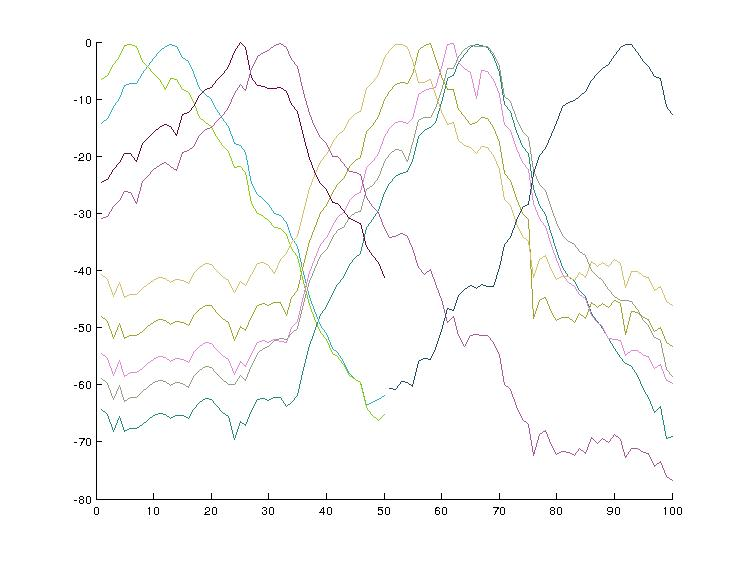
\includegraphics[scale=0.4]{localization}\caption{Localization\label{fig:Localization}}

\par\end{centering}

\end{figure}
\begin{figure}[H]


\begin{centering}
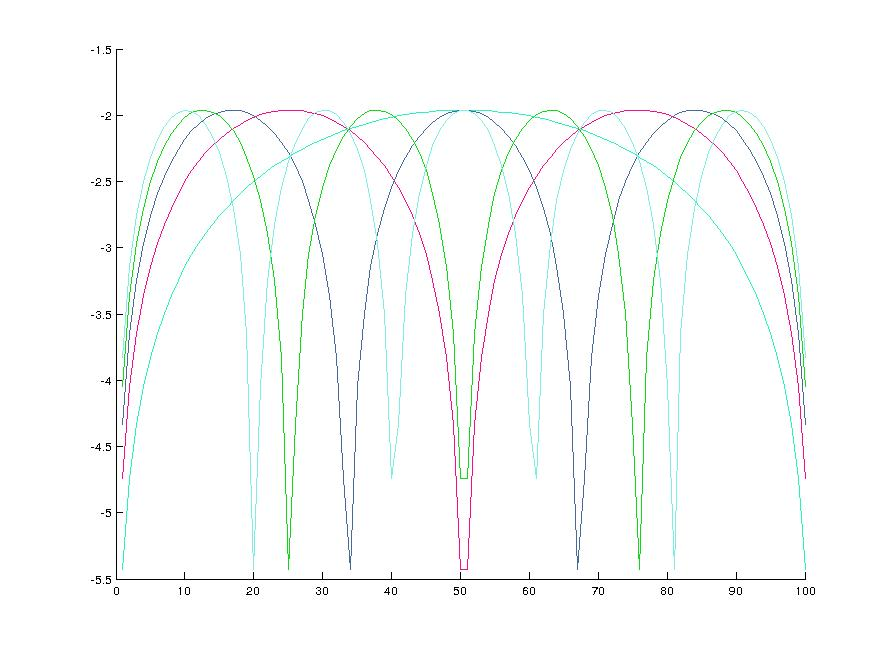
\includegraphics[scale=0.3]{localization_2}\caption{Localization for $\nabla^{2}$\label{fig:Localization-for}}

\par\end{centering}

\end{figure}
\begin{algorithm}[H]


\begin{lstlisting}[language=Matlab]
t=randn(1,100); t1=randn(1,99); T = diag(t)+diag(t1,1)+diag(t1,-1);
[V,D]=eig(T);
figure; axes; hold on;
for i=1:10
    plot(1:100,log(abs(V(:,i))),'color',[rand rand rand]);
end
W = abs(V) >= 10.^(-10); sum(W(:))/10000
% part 2
T = diag(2.*ones(1,100))+diag(-ones(1,99),-1)+diag(-ones(1,99),1);
[V,D]=eig(T);
figure; axes; hold on;
for i=1:5
    plot(1:100,log(abs(V(:,i))),'color',[rand rand rand]);
end
W = abs(V) >= 10.^(-10); sum(W(:))/10000
\end{lstlisting}
\caption{Localization source\label{alg:Localization-source}}


\end{algorithm}

\item [32.2]Gauss-Legendre Quadrature

\begin{enumerate}
\item Do I get extra credit for getting it down to 4 lines? Algorithm appears
in Algorithm \ref{alg:Gauss-Legendre-Quadrature}. 
\begin{algorithm}[H]
\begin{centering}
\begin{lstlisting}
[Q,D]=eig(diag(.5./sqrt(1-(2*(1:n-1)).^(-2)),1)+diag(.5./sqrt(1-(2*(1:n-1)).^(-2)),-1));
x = diag(D);
w = 2*(Q(1,:).^2);
I = dot(w,f(x));
\end{lstlisting}
\caption{Gauss-Legendre Quadrature\label{alg:Gauss-Legendre-Quadrature}}

\par\end{centering}

\end{algorithm}

\item $I_{4}\left(e^{x}\right)=2.350402092156378$ and results of $\log\left(\left|I\left(e^{x}\right)-I_{n}\left(e^{x}\right)\right|\right)$
appear in figure \ref{fig:Gauss-Legendre-Quad} 
\begin{figure}[H]


\begin{centering}
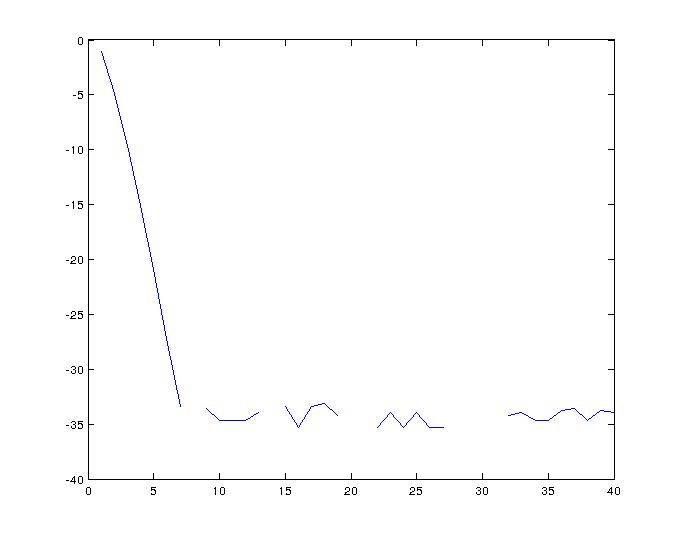
\includegraphics[scale=0.3]{gauss_quad}\caption{Gauss-Legendre Quad $e^{x}$\label{fig:Gauss-Legendre-Quad}}

\par\end{centering}

\end{figure}
Obviously the error in approximating the integral by the quadrature
goes to zero very quickly.
\item The integral of $e^{\left|x\right|}$
\[
\int_{-1}^{1}e^{\left|x\right|}dx=2\int_{0}^{1}e^{x}dx=2\left(e-1\right)
\]
The results of the comparison appear in figure \ref{fig:Gauss-Legendre-Quad-1}.
The error goes to zero slowly and erratically probably because $e^{\left|x\right|}$
is not differentiable at $x=0$. 
\begin{figure}[H]
\centering{}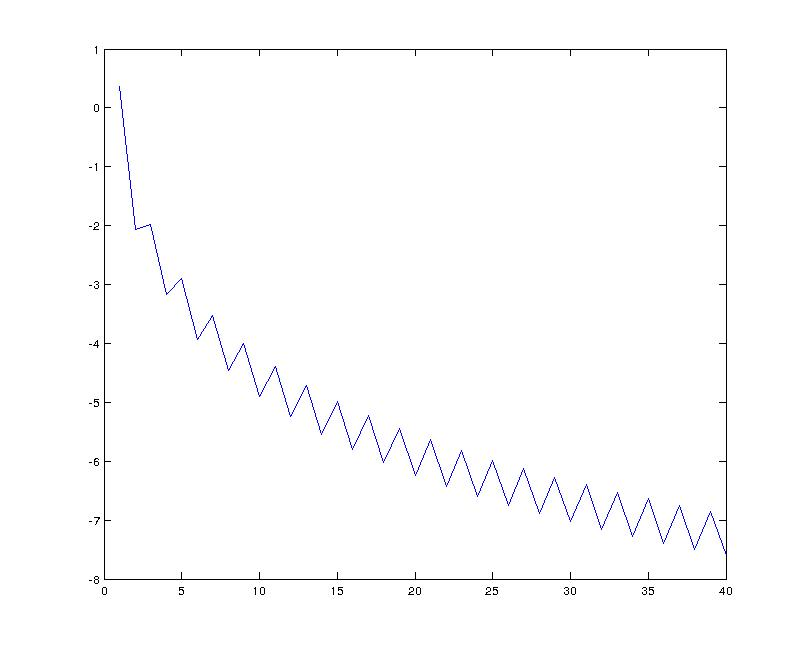
\includegraphics[scale=0.3]{gauss_quad2}\caption{Gauss-Legendre Quad $e^{x}$\label{fig:Gauss-Legendre-Quad-1}}
\end{figure}

\end{enumerate}
\item [38.6]Source appears in algorithm \ref{alg:Conjugate-gradients}.
Log plot appears in figure \ref{fig:Conjugate-gradients-log}. For
some reason gradient descent hits a brick wall in the minimization.
Conjugate gradients doesn't and improves quickly but eventually (at
about iteration 80) stops improving as well. 
\begin{algorithm}
\begin{lstlisting}[language=Matlab,basicstyle={\footnotesize},tabsize=4]
A=diag(1:100)+diag(ones(1,99),1)+diag(ones(1,99),-1);
b=ones(100,1);
CGx={};CGr={};CGp={};
CGx{1} = zeros(100,1); CGr{1} = b; CGp{1} = CGr{1};
for n=2:100
    an = (CGr{n-1}'*CGr{n-1})/(CGp{n-1}'*A*CGp{n-1});
    CGx{n} = CGx{n-1} + an.*CGp{n-1};
    CGr{n} = CGr{n-1} - an.*(A*CGp{n-1});
    bn = (CGr{n}'*CGr{n})/(CGr{n-1}'*CGr{n-1});
    CGp{n} = CGr{n} + bn.*CGp{n-1};
end

SDx={};SDr={};
SDx{1} = zeros(100,1); SDr{1} = b; 
for n=2:100
    an = (SDr{n-1}'*SDr{n-1})/(SDr{n-1}'*A*SDr{n-1});
    SDr{n} = SDr{n-1} - an.*(A*SDr{n-1});
    SDx{n} = SDx{n-1} + an.*SDr{n}; end

ka = max(eig(A))/min(eig(A));
plot(1:100,cellfun(@(x)(log(norm(x))),CGr),'-.r*',...
    	1:100,cellfun(@(x)(log(norm(x))),cellfun(@(x)(b-A*x),CGx,'UniformOutput',false)),'--mo',...
    	1:100,cellfun(@(x)(log(norm(x))),SDr),':bs',...
    	1:100,log(2*((sqrt(ka)-1)/(sqrt(ka)+1)).^(1:100)),':gx')
legend('est resid norms CG','act resid norms CG','resid norms SD','k');
\end{lstlisting}


\caption{Conjugate gradients\label{alg:Conjugate-gradients}}


\end{algorithm}
\begin{figure}[H]


\centering{}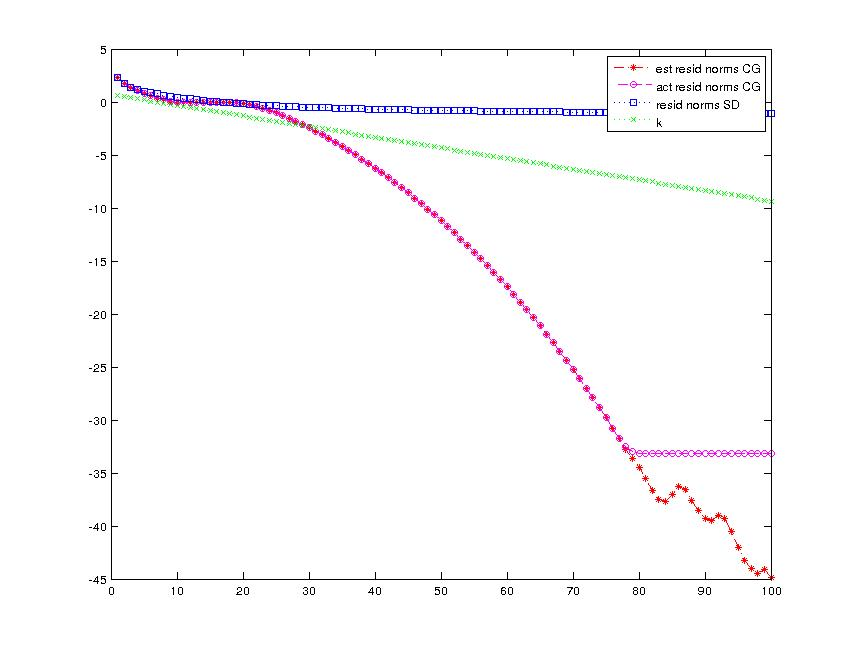
\includegraphics[scale=0.5]{cg}\caption{Conjugate gradients log plot\label{fig:Conjugate-gradients-log}}
\end{figure}
\end{enumerate}

\end{document}
